In the introduction, we showed our choreography language via an
example. We now formalise our language by giving its syntax and
semantics. For the sake of clarity, we slightly change the syntax with
respect to the syntax of our tool, adopting a more process-algebra
format.

\subsection{Syntax} 
%
Let $\role p$ range over a (possibly infinite) set of module names
$\mathcal R$, $x$ over a (possibly infinite) set of variables $\Var$,
and $v$ over a (possibly infinite) set of values $\Val$.
%
Choreographies, the key component of our language, are defined by the
following syntax:
%
\begin{displaymath}\small
  \begin{array}{llllllllllll}
    C & ::= &      & \interact{p}{\role p_1,\ldots,\role p_n} & \text{(interaction)}\\[1mm]
      % &     & \mid & \allsynch pGiI & \text{(non-deterministic sync)}\\
      &     & \mid & \ifTE {E}{p}{C_1}{C_2} & \text{(conditional)}\\[1mm]
      &     & \mid & X     & \text{(recursive call)}\\[1mm]
      &     & \mid & \CEnd & \text{(inact)}
    % \\
    %   &     & \mid & \textsf{foreach } E\ u@{\role p}[i];\, C & \text{(foreach)}
    \\[2mm]
    \defin \ & ::= & & X\stackrel{\mathsf{def}}{=} C,\ \defin 
                     \quad \mid \quad \emptyset & \text{(definitions)}
    \\[2mm]
    u     & ::=  && (x' = E)\ \&\ u \quad\mid\quad    (x' = E) & \text{(assignments)}\\[2mm]
    E, g  & ::=  && f(\tilde E)\quad\mid\quad x\quad\mid\quad v & \text{(expressions)}
  \end{array}
\end{displaymath}
%
% We comment the various constructs.
The syntactic category $C$ denotes choreographic programs. The
interaction term
$\role p\rightarrow \{\role p_1,\ldots,\role
p_n\}:\,\Sigma\{\lambda_j: x_j=E_j.\ C_j\}_{j\in J}$ denotes an
interaction initiated by module $\role p$ with modules $\role p_i$'s
(for $\role p$ and all $\role p_i$ distinct). A choreography specifies
what interaction must be executed next, shifting the focus from what
can happen to what must happen. When the interaction happens, one of
the $j$ branches is selected as a continuation. Branching is a random
move: the number $\lambda_j\in\mathbb R$ denotes either a probability
or a rate. This will depend on the language we wish to use. In the
case of probabilities, it must be the case that $0\leq\lambda_j\leq 1$
and $\Sigma_j\lambda_j=1$. Once a branch $j$ is taken, the
choreography will execute some assignments $u_j$. A single assignment
has the syntax $(x' = E)$ meaning that the value obtained by
evaluating expression $E$ is assigned to variable $x$; assignments can
be concatenated with the operator $\&$.  Note that $x'$ is used for an
assignment to $x$: here, we follow the syntax adopted in PRISM
(see~\S~\ref{sec:prism}). Expressions are obtained by applying some
unspecified functions to other expressions or, as base terms, i.e.,
variables and values (denoted by $v$).
%

The term $\ifTE {E}{p}{C_1}{C_2}$ denotes a system where module
  $\role p$ evaluates the guard $E$ (which can contain variables
  located at other modules) and then (deterministically) branches
  accordingly.  The term $X$ is a (possibly recursive) procedure call:
  in the semantics, we assume that such procedure names are defined
  separately.  The term $\CEnd$ denotes the system finishing its
  computation.

\bigskip


\subsection{Semantics.} The semantics of a choreography is a relation
that captures how the values assigned to variables are modified when
the various modules synchronise with each other. Similar to the
operational semantics of imperative languages, we define a state,
denoted by $S$, as a mapping from variables to values, i.e.,
$S: \Var \rightarrow\Val$.
%

Given a state, substitution allows to modify some of its values:
%
\begin{definition}
  Given a value $v$ and a variable $x$, a substitution $[v/x]$ is an
  update on a state, i.e., $\small S[v/x] (y)= \left\{
  \begin{array}{ll} 
    v    & \text{ if } y=x\\ 
    S(y) & \text{ otherwise}
  \end{array} \right.
$
%
Then, the update $S[u]$ is such that
$S[x'=E\ \&\ u] = S[\eval ES/x][u]$ and $S[x'=E] = S[\eval ES/x]$,
where $\eval ES$ is an unspecified (decidable) evaluation of the
expression $E$ in the state $S$.
\end{definition}

Given the set of all possible states $\mathcal S$ and a set of
definitions $\defin$ of the form $X\stackrel{\mathsf{def}}{=} C$, we
can define the operational semantics of choreographies as the minimal
relation
$\red{}\!\!\!\!^\defin\subseteq \mathcal S\times C\times \mathbb
R\times \mathcal S\times C$ such that (we omit $\defin$ if not
relevant):
\begin{displaymath}\small
  \begin{array}{l@{\quad}llll}
    \textsf{(Interact)} &
    (S, \interact{p}{\role p_1,\ldots,\role p_n}) 
    % \red{\Sigma_{(S[u_j],C_j)=(S',C')}\lambda_j}
    % (S', C') 
    \red{\lambda_j}
    (S[u_j], C_j) 
    \\[1mm]
    \textsf{(IfThenElseT)} &
    \eval ES = \mathsf{tt} \quad\Rightarrow\quad
    (S,\ifTE {E}{p}{C_1}{C_2}) 
    \red{1}
    (S, C_1)
    \\[1mm]
    \textsf{(IfThenElseF)} &
    \eval ES = \mathsf{ff} \quad\Rightarrow\quad
    (S,\ifTE {E}{p}{C_1}{C_2}) 
    \red{1}
    (S, C_2)
    \\[1mm]
    \textsf{(Call)} &
    X\stackrel{\mathsf{def}}{=} C\in\defin \quad\Rightarrow\quad (S, X) \red{1}(S,C)
  \end{array}
\end{displaymath}
The transition relation is a Discrete Time Markov Chain (DTMC) or a
Continuous Time Markov Chain (CTMC) depending on whether we use
probabilities or rates in the branching construct. Note that states of
the Markov chain are the pairs $(S,C)$, while the transitions are
given by the relation $\red{}$.
%

% Below, we look at two corner-case examples.
\begin{example}
  Consider the following choreography:
  \begin{displaymath}
    \begin{array}{lll}
      C \ {=}\ \interactBase{p}{q}\ \lambda_1: (x'=1);\quad \interactBase{p}{q}\ \lambda_2: (x'=1);\CEnd
    \end{array}
  \end{displaymath}
  The semantics of $C$ starting from a state in which $S(x)=S(y)=0$
  can be depicted as follows (for
  $C'= \interactBase{p}{q}\ \lambda_1: (x'=1);\CEnd$):

\bigskip
\begin{comment}
\begin{tikzpicture}\small
    \node[state, initial] (1) 
    {\tiny$\begin{array}{c}
      C \\ x=0
    \end{array}$};
    \node[state, right of=1, xshift=3cm] (2) 
        {\tiny$\begin{array}{c}
      C' \\ x=1
    \end{array}$};
    \node[state, right of=2, xshift=3cm] (3) 
        {\tiny$\begin{array}{c}
      \CEnd \\ x=1
    \end{array}$};
     \draw[->]   (1) edge[above] node{$\lambda_1$} (2)
             (2) edge[below] node{$\lambda_2$} (3)
     ;
\end{tikzpicture}
\end{comment}
\begin{figure}[!h]
  \centering
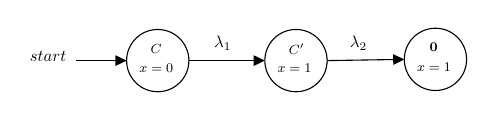
\begin{tikzpicture}[x=0.75pt,y=0.75pt,yscale=-1,xscale=1,scale=0.6, every node/.style={scale=0.6}]
  %uncomment if require: \path (0,300); %set diagram left start at 0, and has height of 300
  %Shape: Circle [id:dp1991798631163264] 
  \draw   (219,126) .. controls (219,112.19) and (230.19,101) .. (244,101) .. controls (257.81,101) and (269,112.19) .. (269,126) .. controls (269,139.81) and (257.81,151) .. (244,151) .. controls (230.19,151) and (219,139.81) .. (219,126) -- cycle ;
  %Shape: Circle [id:dp10467411334622834] 
  \draw   (330,126) .. controls (330,112.19) and (341.19,101) .. (355,101) .. controls (368.81,101) and (380,112.19) .. (380,126) .. controls (380,139.81) and (368.81,151) .. (355,151) .. controls (341.19,151) and (330,139.81) .. (330,126) -- cycle ;
  %Shape: Circle [id:dp3427541367043958] 
  \draw   (442,125) .. controls (442,111.19) and (453.19,100) .. (467,100) .. controls (480.81,100) and (492,111.19) .. (492,125) .. controls (492,138.81) and (480.81,150) .. (467,150) .. controls (453.19,150) and (442,138.81) .. (442,125) -- cycle ;
  %Straight Lines [id:da18643758642972075] 
  \draw    (178,126) -- (216,126) ;
  \draw [shift={(219,126)}, rotate = 180] [fill={rgb, 255:red, 0; green, 0; blue, 0 }  ][line width=0.08]  [draw opacity=0] (8.93,-4.29) -- (0,0) -- (8.93,4.29) -- cycle    ;
  %Straight Lines [id:da45756471809990495] 
  \draw    (269,126) -- (327,126) ;
  \draw [shift={(330,126)}, rotate = 180] [fill={rgb, 255:red, 0; green, 0; blue, 0 }  ][line width=0.08]  [draw opacity=0] (8.93,-4.29) -- (0,0) -- (8.93,4.29) -- cycle    ;
  %Straight Lines [id:da4059508932352085] 
  \draw    (380,126) -- (439,125.05) ;
  \draw [shift={(442,125)}, rotate = 179.08] [fill={rgb, 255:red, 0; green, 0; blue, 0 }  ][line width=0.08]  [draw opacity=0] (8.93,-4.29) -- (0,0) -- (8.93,4.29) -- cycle    ;
  
  % Text Node
  \draw (228,127.4) node [anchor=north west][inner sep=0.75pt]  [font=\footnotesize]  {$x=0$};
  % Text Node
  \draw (237,111.4) node [anchor=north west][inner sep=0.75pt]  [font=\footnotesize]  {$C$};
  % Text Node
  \draw (339,127.4) node [anchor=north west][inner sep=0.75pt]  [font=\footnotesize]  {$x=1$};
  % Text Node
  \draw (348,111.4) node [anchor=north west][inner sep=0.75pt]  [font=\footnotesize]  {$C'$};
  % Text Node
  \draw (451,126.4) node [anchor=north west][inner sep=0.75pt]  [font=\footnotesize]  {$x=1$};
  % Text Node
  \draw (461,110.4) node [anchor=north west][inner sep=0.75pt]  [font=\footnotesize]  {$\mathbf{0}$};
  % Text Node
  \draw (140,117) node [anchor=north west][inner sep=0.75pt]   [align=left] {$\displaystyle start$};
  % Text Node
  \draw (288,105) node [anchor=north west][inner sep=0.75pt]   [align=left] {$\displaystyle \lambda _{1}$};
  % Text Node
  \draw (397,105) node [anchor=north west][inner sep=0.75pt]   [align=left] {$\displaystyle \lambda _{2}$};
  \end{tikzpicture}
\end{figure}
\end{example}


\begin{example}\label{example2}
  Consider the following definition:
  \begin{displaymath}
    \begin{array}{lll}
      C \stackrel{\mathsf{def}}{=} \interactBase{p}{q}
      \left\{
      \begin{array}{lll}
        \lambda_1: (x'=1)\&(y'=2);\ C
        \\
        \lambda_2: (x'=3)\&(y'=1);\ C
      \end{array}
      \right.
    \end{array}
  \end{displaymath}
The semantics of $C$ starting from a state in which $S(x)=S(y)=0$ can
be depicted as follows:

\bigskip
\begin{comment}
\begin{tikzpicture}\small
    \node[state, initial] (1) 
    {\tiny$\begin{array}{c}
      C \\ x=0\\ y=0
    \end{array}$};
    \node[state, right of=1, xshift=4cm] (2) 
        {\tiny$\begin{array}{c}
      C \\ x=1\\ y=2
    \end{array}$};
    \node[state, below right of=1, xshift=1.8cm] (3) 
        {\tiny$\begin{array}{c}
      C \\ x=3\\ y=1
    \end{array}$};
     \draw [->]  (1) edge[above, bend left] node{$\lambda_1$} (2)
             (1) edge[below, bend right] node{$\lambda_2$} (3)
             (2) edge[loop right] node{$\lambda_1$} (2)
             (3) edge[loop below] node{$\lambda_2$} (3)
             (2) edge[below, bend left] node{$\lambda_2$} (3)
             (3) edge[above] node{$\lambda_1$} (2)
     ;
\end{tikzpicture}
\end{comment}
\begin{figure}[h]
  \centering
  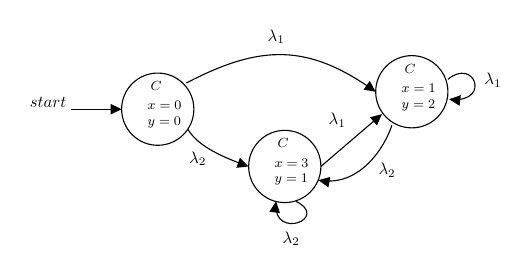
\begin{tikzpicture}[x=0.75pt,y=0.75pt,yscale=-1,xscale=1,scale=0.6, every node/.style={scale=0.6}]
    %uncomment if require: \path (0,448); %set diagram left start at 0, and has height of 448
    %Shape: Circle [id:dp07054898935668796] 
    \draw   (235,148) .. controls (235,131.98) and (247.98,119) .. (264,119) .. controls (280.02,119) and (293,131.98) .. (293,148) .. controls (293,164.02) and (280.02,177) .. (264,177) .. controls (247.98,177) and (235,164.02) .. (235,148) -- cycle ;
    %Straight Lines [id:da7347994961242792] 
    \draw    (194,148) -- (232,148) ;
    \draw [shift={(235,148)}, rotate = 180] [fill={rgb, 255:red, 0; green, 0; blue, 0 }  ][line width=0.08]  [draw opacity=0] (8.93,-4.29) -- (0,0) -- (8.93,4.29) -- cycle    ;
    %Shape: Circle [id:dp22606672052423815] 
    \draw   (337,194) .. controls (337,177.98) and (349.98,165) .. (366,165) .. controls (382.02,165) and (395,177.98) .. (395,194) .. controls (395,210.02) and (382.02,223) .. (366,223) .. controls (349.98,223) and (337,210.02) .. (337,194) -- cycle ;
    %Shape: Circle [id:dp004245899794039332] 
    \draw   (439,134) .. controls (439,117.98) and (451.98,105) .. (468,105) .. controls (484.02,105) and (497,117.98) .. (497,134) .. controls (497,150.02) and (484.02,163) .. (468,163) .. controls (451.98,163) and (439,150.02) .. (439,134) -- cycle ;
    %Curve Lines [id:da36630684284037396] 
    \draw    (287,127) .. controls (347.09,95.48) and (384.85,95.98) .. (436.62,132.31) ;
    \draw [shift={(439,134)}, rotate = 215.64] [fill={rgb, 255:red, 0; green, 0; blue, 0 }  ][line width=0.08]  [draw opacity=0] (8.93,-4.29) -- (0,0) -- (8.93,4.29) -- cycle    ;
    %Curve Lines [id:da4071587559359209] 
    \draw    (288,164) .. controls (293.85,172.78) and (302.55,181.55) .. (334.5,193.11) ;
    \draw [shift={(337,194)}, rotate = 199.44] [fill={rgb, 255:red, 0; green, 0; blue, 0 }  ][line width=0.08]  [draw opacity=0] (8.93,-4.29) -- (0,0) -- (8.93,4.29) -- cycle    ;
    %Straight Lines [id:da7160141088008605] 
    \draw    (395,194) -- (441.72,153.95) ;
    \draw [shift={(444,152)}, rotate = 139.4] [fill={rgb, 255:red, 0; green, 0; blue, 0 }  ][line width=0.08]  [draw opacity=0] (8.93,-4.29) -- (0,0) -- (8.93,4.29) -- cycle    ;
    %Curve Lines [id:da7788168425777569] 
    \draw    (452,161) .. controls (446.18,178.46) and (427.19,209.09) .. (395.93,205.44) ;
    \draw [shift={(393,205)}, rotate = 10.3] [fill={rgb, 255:red, 0; green, 0; blue, 0 }  ][line width=0.08]  [draw opacity=0] (8.93,-4.29) -- (0,0) -- (8.93,4.29) -- cycle    ;
    %Curve Lines [id:da05888759989591952] 
    \draw    (375,222) .. controls (402.16,235.58) and (357.81,252.92) .. (358.78,224.75) ;
    \draw [shift={(359,222)}, rotate = 97.13] [fill={rgb, 255:red, 0; green, 0; blue, 0 }  ][line width=0.08]  [draw opacity=0] (8.93,-4.29) -- (0,0) -- (8.93,4.29) -- cycle    ;
    %Curve Lines [id:da66106493809224] 
    \draw    (497,124) .. controls (518.34,106.54) and (531.21,141.77) .. (500.93,140.25) ;
    \draw [shift={(498,140)}, rotate = 6.71] [fill={rgb, 255:red, 0; green, 0; blue, 0 }  ][line width=0.08]  [draw opacity=0] (8.93,-4.29) -- (0,0) -- (8.93,4.29) -- cycle    ;
    
    % Text Node
    \draw (248,138.4) node [anchor=north west][inner sep=0.75pt]  [font=\footnotesize]  {$ \begin{array}{l}
    x=0\\
    y=0
    \end{array}$};
    % Text Node
    \draw (257,124.4) node [anchor=north west][inner sep=0.75pt]  [font=\footnotesize]  {$C$};
    % Text Node
    \draw (160,137) node [anchor=north west][inner sep=0.75pt]   [align=left] {$\displaystyle start$};
    % Text Node
    \draw (350,184.4) node [anchor=north west][inner sep=0.75pt]  [font=\footnotesize]  {$ \begin{array}{l}
    x=3\\
    y=1
    \end{array}$};
    % Text Node
    \draw (359,170.4) node [anchor=north west][inner sep=0.75pt]  [font=\footnotesize]  {$C$};
    % Text Node
    \draw (452,124.4) node [anchor=north west][inner sep=0.75pt]  [font=\footnotesize]  {$ \begin{array}{l}
    x=1\\
    y=2
    \end{array}$};
    % Text Node
    \draw (461,110.4) node [anchor=north west][inner sep=0.75pt]  [font=\footnotesize]  {$C$};
    % Text Node
    \draw (351,83) node [anchor=north west][inner sep=0.75pt]   [align=left] {$\displaystyle \lambda _{1}$};
    % Text Node
    \draw (400,150) node [anchor=north west][inner sep=0.75pt]   [align=left] {$\displaystyle \lambda _{1}$};
    % Text Node
    \draw (525,118) node [anchor=north west][inner sep=0.75pt]   [align=left] {$\displaystyle \lambda _{1}$};
    % Text Node
    \draw (288,181) node [anchor=north west][inner sep=0.75pt]   [align=left] {$\displaystyle \lambda _{2}$};
    % Text Node
    \draw (440,190) node [anchor=north west][inner sep=0.75pt]   [align=left] {$\displaystyle \lambda _{2}$};
    % Text Node
    \draw (363,245) node [anchor=north west][inner sep=0.75pt]   [align=left] {$\displaystyle \lambda _{2}$};
    
    
    \end{tikzpicture}
  \end{figure}
\end{example}


\subsection{Other language constructs}
%
The attentive reader may have noticed that the syntax used in our
introductory example includes language constructs that are not part of
the formal syntax given above. Given the nature of our language, these
constructs are purely syntactic sugar and can be easily
encoded. Below, we discuss each of them:
% 
\begin{itemize}

\item {\em Parametric modules.} In our implemented language, modules
  can be parameterised (indexed) as done in PRISM. We denote
  parameterised roles as $\role p[n]$ for $n$ ranging some finite set
  $N$.
  %
  As an example, the choreography
  \[\interactBase {p[i]}{q[i]}:\lambda:U;\quad 
    \interactBase r{q[i]}:\lambda:U;\quad \CEnd
  \]
  can be easily encoded as:
  \[
    \begin{array}{llll}
      \interactBase {p1}{q1}:\lambda:U;\quad \\
      \interactBase {p2}{q2}:\lambda:U;\quad \\
      \interactBase {p3}{q3}:\lambda:U;\quad \\
      \interactBase r{q1,q2,q3}:\lambda:U;\quad \CEnd
    \end{array}
  \]
  Note that if the second parametric interaction were
  $\interactBase {q[i]}r:\lambda:U;\quad \CEnd$, then we would have to
  turn around the synchronisation. \marco{ADELE, COSA SUCCEDE
    NELL'IMPLEMENTAZIONE?}
  %
  Additionally, the choreography
  \[\interactBase {p[i]}{q[i]}:\lambda:U;\quad 
    \interactBase {q[i+1]}{p[i]}:\lambda:U;\quad \CEnd
  \]
  can be encoded in our model language as
  \[
    \begin{array}{llll}
      \interactBase {p1}{q1}:\lambda:U;\quad \\
      \interactBase {q2}{p1}:\lambda:U;\quad \\
      \interactBase {p2}{q2}:\lambda:U;\quad \\
      \interactBase {q3}{p2}:\lambda:U;\quad \\
      \interactBase {p3}{q3}:\lambda:U;\quad \\
      \interactBase {q1}{p3}:\lambda:U;\quad  \CEnd
    \end{array}
  \]
  Given that parameters range over a finite set, this operation is
  redundant as far as the theory is concerned.\marco{We need to
    discuss this, I'm not really sure the semantics is equivalent}

\item {\em The {\sf foreach} construct.} The use of parametric modules
  can be further facilitated by introducing syntactic sugar that
  allows iteration over the set of indices that parameterise these
  modules. To this end, our language implementation includes the
  construct $\textsf{foreach } E(i)\ u@A[i];, C$. \marco{Adele, check
    syntax?}  This construct enables the expression $E(i)$ to range
  over a set of indices, which can then be used in $u@A[i]$. In
  essence, it provides a more concise and readable way to express
  operations over multiple indexed modules. Notably, this construct
  can be encoded explicitly by numbering the modules manually,
  provided that the indices are known at compile time rather than
  determined dynamically at runtime.


\item {\em Non-deterministic Synchronisation.}  Our implementation
  supports the non-deterministic synchronisation language construct
  $\allsynch pGiI$, where $G$ has the form $\chorcommand g\lambda
  u$. The core idea behind this construct is to enable a set of roles,
  denoted by $\role{p_i}$, to synchronise while allowing each role to
  non-deterministically select from a range of possible local
  actions. This provides a structured mechanism for defining
  interactions where multiple roles must coordinate, but their precise
  behaviour may vary dynamically (with a certain probability
  distribution/rate).

  A key advantage of this construct is its compactness and readability
  in specifying synchronised interactions. For instance, in a scenario
  where two roles, $\role{p}$ and $\role{q}$, participate in a
  synchronised exchange, the $\allsynchName$ syntax allows for a
  concise definition of conditions under which each role updates its
  state. This avoids the need for manually encoding synchronisation
  through nested conditional constructs.
  % 
  Despite its expressiveness, the $\allsynchName$ construct does not
  introduce new semantics but serves as syntactic sugar for an
  equivalent formulation.  In fact, $\allsynchName$ can be rewritten
  using a series of nested $\mathtt{if\text{-}then\text{-}else}$
  constructs, ensuring that the synchronisation conditions are met
  before proceeding with the interaction. For example, consider the
  non-deterministic synchronisation between roles $\role p$ and
  $\role q$: \marco{update with Adele with more commands for each
    role}
  %
  \begin{displaymath}
    % C \stackrel{\mathsf{def}}{=} 
    %
    \allsynchName\left\{
      \begin{array}{lll}
        \role{p} : (x=1) \rightarrow 1 : (x'=100) \\
        \role{q} : (y=1) \rightarrow 1 : (y'=0)
      \end{array}
    \right\} ; \CEnd
  \end{displaymath}
  %
  This construct provides a compact and structured way to define
  synchronized interactions. However, it can be rewritten without
  using the $\allsynchName$ syntax by explicitly handling conditions
  using the $\mathtt{if\text{-}then\text{-}else}$ construct:
  
  \begin{displaymath}
    \begin{array}{ll}
      % C' \stackrel{\mathsf{def}}{=}
      & \mathtt{if}\ (x=1)@\role {p}\ \mathtt{then}\\
      & \quad \mathtt{if}\ (y=1)@\role {q}\ \mathtt{then}\\
      & \quad \quad \interactBase{p}{q}\ 1 : (x'=100)\&(y'=0);\CEnd \\
      & \quad \mathtt{else}\ \CEnd \\
      & \mathtt{else}\ \CEnd
    \end{array}
  \end{displaymath}
  %
  The two formulations are equivalent, with the $\allsynchName$ syntax
  acting as syntactic sugar for a structured and readable
  representation of synchronization. The expanded version using
  $\mathtt{if\text{-}then\text{-}else}$ makes explicit the conditional
  execution of interactions but retains the same behaviour.

  By incorporating $\allsynchName$, our implementation streamlines the
  specification of non-deterministic synchronisation while preserving
  its precise operational semantics, ultimately enhancing both clarity
  and usability in defining distributed interactions.
\end{itemize}

  



%%% Local Variables: 
%%% mode: latex
%%% TeX-master: "main"
%%% End:
